\documentclass{article}
\usepackage{arxiv}
\usepackage[utf8]{inputenc}
\usepackage[T1]{fontenc}
\usepackage{natbib}
\usepackage{hyperref}
\usepackage{url}
\usepackage{booktabs}
\usepackage{amsfonts}
\usepackage{amsmath}
% \usepackage{nicefrac}  % not available in BasicTeX
\usepackage{microtype}
\usepackage{graphicx}
\usepackage{xcolor}
\usepackage{caption}

\title{Structure Beats Scale: How Structured Review Outperforms Brute-Force Generation in LLM Code Synthesis}

\renewcommand{\shorttitle}{Structure Beats Scale}
\renewcommand{\headeright}{}

\author{
  Stevo Ledbetter \\
  Independent Researcher \\
  \texttt{stevo@smledbetter.com}
}

\date{March 2026}

\begin{document}
\maketitle

% ============================================================
\begin{abstract}
The standard strategy for improving LLM code generation is to generate more samples and pick the best one. Across over 3,000 experimental runs on 60 competitive programming problems, 25 HumanEval problems, and 25 MBPP problems, spanning three code benchmarks, three generator models, and 17 inference-time compute allocation strategies, I find that structured review pipelines---specifically a hybrid of multiple generations with independent reviews on each---generally dominate the Pareto frontier of pass rate versus cost. On a calibration set of 30 competitive programming problems, the best hybrid configuration (C13: 3 generations + 2 reviews each) achieves 85.1\% pass rate (SE=5.7\%) at \$0.141/problem, compared to 82.8\% (SE=5.6\%) at \$0.221/problem for best-of-7 generation (C16). The 2.3 percentage point gap is not statistically significant ($p=0.53$); the argument for C13 over C16 is Pareto dominance---C13 is both cheaper and higher in point estimate---not statistical separation. The ordering C0~(baseline) $<$ C9~(debate) $<$ C13~(hybrid) replicates on 30 held-out problems (C0=38.7\%, C9=51.5\%, C13=55.6\%; C0 vs C13: $p=0.002$). The ordering holds across two alternative generators---Qwen 2.5 Coder 32B and DeepSeek V3---but a matched-fixer experiment reveals that the mechanism differs by generator capability: when the fixer matches the generator (instead of always being Sonnet), Qwen pipelines collapse to 0\% while DeepSeek pipelines retain their gains (C9=41.9\%, C13=51.8\%). The DeepSeek result suggests the review pipeline genuinely works for capable generators; the Qwen result is consistent with the gains coming from the strong fixer rather than the review structure, though a floor effect (Qwen=0\% at baseline) limits interpretation. On HumanEval and MBPP combined, the result is unambiguous: C13=93.0\% vs C16=64.7\% ($p=0.0002$). A temperature sensitivity analysis confirms the result is robust to sampling parameter variation. When you have budget for more than one LLM call, the evidence favors spending it on review structure over more independent samples---achieving Pareto-dominant performance (equal or higher pass rate at lower cost) across all tested conditions---provided the fixer is capable enough to act on review feedback.
\end{abstract}

% ============================================================
\section{Introduction}

You have an LLM that generates code and gets the right answer about half the time (52.0\% on the calibration set). You have budget for more API calls---what do you do with them?

The obvious answer---the one most practitioners reach for---is to generate more solutions and pick the best. Best-of-$N$ sampling. It is the path of least architectural resistance: no new prompts to write, no review logic to build, no multi-model orchestration to debug. Just crank up $N$ and let probability do the work. And it does work, up to a point. \citet{chen2021evaluating} showed that pass@$k$ scales predictably with $k$ for Codex. \citet{li2022competition} demonstrated that massive-scale generation paired with execution-based filtering and clustering (AlphaCode) extends this further. The entire inference-time compute scaling literature---from \citet{wang2023selfconsistency}'s self-consistency to \citet{snell2024scaling}'s compute-optimal scaling laws---implicitly treats generation diversity as the primary lever.

That's not the interesting part. The interesting part is what happens when you spend the same budget on \emph{structure} instead of \emph{volume}. I ran 17 experimental conditions across 6 strategy families---baseline, generation-only, review-heavy, debate, iterative fix loops, and hybrid generation-plus-review---on 60 competitive programming problems, then replicated on held-out problems, validated across three generator models, and generalized to two additional benchmarks. The core finding on calibration data is clean: structured review pipelines dominate the Pareto frontier of pass rate versus cost. Brute-force generation scaling never lands on it. The ordering C0~(baseline) $<$ C9~(debate) $<$ C13~(hybrid) holds across every experimental condition I tested, though the gap between C9 and C13 is not statistically significant after correction on any individual dataset. The evidence is strongest on the calibration set and cross-domain benchmarks, and directional on held-out competitive programming problems where smaller sample sizes limit statistical power.

This paper makes three contributions. First, I establish a Pareto frontier for inference-time compute allocation in code generation, showing that review-augmented strategies dominate generation-only strategies at every cost level on the calibration set (Section~\ref{sec:results}). Second, I demonstrate that the ordering replicates on held-out problems (Spearman $\rho=0.786$, $p=0.036$), generalizes across generators with fundamentally different capability profiles, and transfers to standard benchmarks---with explicit accounting of where the evidence is strong and where it is directional (Section~\ref{sec:replication}). Third, I show that structured review improves individual pipeline quality---not just selection---by comparing pass@1 rates between reviewed and unreviewed multi-generation configurations (Section~\ref{sec:whyitworks}). The remainder of the paper is organized as follows: Section~\ref{sec:related} covers related work, Section~\ref{sec:method} describes the experimental method, Sections~\ref{sec:results}--\ref{sec:whyitworks} present results, Section~\ref{sec:ablations} reports ablations and strategy family analysis, Section~\ref{sec:limitations} addresses limitations, and Section~\ref{sec:conclusion} concludes.

% ============================================================
\section{Related Work}
\label{sec:related}

\subsection{Inference-Time Compute Scaling}

The question of how to spend inference-time compute has received increasing attention as LLM capabilities have improved. \citet{snell2024scaling} established compute-optimal scaling laws showing that the best allocation depends on problem difficulty---easy problems benefit most from sequential revision, while harder problems require balancing revision with parallel sampling. My work extends this by systematically comparing six strategy families on a fixed problem set with full cost accounting, rather than comparing two strategies at a time.

\citet{wang2023selfconsistency} introduced self-consistency, which aggregates multiple chain-of-thought reasoning paths by majority vote. Their insight---that diverse reasoning paths provide a form of ensemble---is related to my generation-only conditions (C3, C6, C11, C16). However, self-consistency operates on reasoning paths for a single answer, while my generation conditions produce independent code solutions evaluated against test suites. The selection mechanism differs fundamentally: majority vote over reasoning versus functional correctness over execution.

\subsection{LLM-Based Code Review and Repair}

The use of LLMs to review and repair generated code has been explored along several axes. \citet{madaan2023selfrefine} proposed Self-Refine, an iterative self-feedback loop where a single model critiques and revises its own output. My iterative conditions (C4, C10, C12, C14) test a similar pattern but with a separate review model, which avoids the self-consistency bias that Self-Refine inherits. \citet{olausson2024selfrepair} found that self-repair gains are often modest or absent once compute cost is accounted for, with the primary bottleneck being the model's limited ability to generate accurate diagnostic feedback on its own code---a finding that motivates my use of separate reviewer models rather than self-review.

\citet{chen2023codet} introduced CodeT, which uses LLM-generated test cases to filter and rank code solutions, achieving a form of automated verification that is complementary to the review approach tested here. My pipeline uses human-written test suites for selection rather than generated tests, which avoids the dual-generation confound but limits applicability to settings where test suites exist.

\citet{shinn2023reflexion} introduced Reflexion, which uses verbal self-reflection on task feedback---including execution results for code tasks---to iteratively improve solutions, and \citet{zhou2024lats} proposed Language Agent Tree Search (LATS), which combines LLM-based evaluation with tree search over action sequences. Both represent alternative architectures for spending inference-time compute on structure rather than volume; my work differs in testing a broader space of strategies on a single benchmark suite with direct cost comparison.

\citet{jimenez2024swebench} introduced SWE-bench, a benchmark of real-world GitHub issues requiring multi-file code changes. My evaluation uses function-level benchmarks (competitive programming, HumanEval, MBPP), which test algorithmic problem-solving rather than software engineering. Whether structured review helps with multi-file, underspecified, real-world code changes is an open question---one that SWE-bench is better positioned to answer than my current setup.

\subsection{Multi-Agent Debate and Deliberation}

\citet{du2023improving} showed that multi-agent debate improves factuality and reasoning in language models by having multiple LLM instances debate answers. \citet{liang2023encouraging} showed that multi-agent debate can promote divergent thinking, finding that moderated disagreement between agents improves reasoning outcomes---though the benefit depends on calibrating the intensity of debate, not simply maximizing disagreement. This is a mechanism my single-turn debate conditions cannot capture. My debate conditions (C2, C9, C15) adapt this paradigm to code generation, where ``debate'' means multiple independent reviewers evaluating the same code and a fixer synthesizing their feedback. The key distinction is that my debate is single-turn and sequential---reviewers do not respond to each other---which is a limitation I address in Section~\ref{sec:limitations}.

\citet{hong2023metagpt} proposed MetaGPT, which assigns structured roles (product manager, architect, project manager, engineer, QA engineer) to collaborating agents for software development. My pipeline instantiates a simpler version of this role differentiation---generator, reviewer, fixer---without the organizational meta-structure. The key difference is that my agents do not communicate with each other; the pipeline is strictly sequential.

\subsection{Code Generation Benchmarks}

I evaluate on competitive programming problems, HumanEval \citep{chen2021evaluating}, and MBPP \citep{austin2021program}. \citet{hendrycks2021apps} introduced APPS, a large-scale coding challenge benchmark with difficulty tiers (introductory, interview, competition); my competitive programming problems occupy a similar niche but are drawn from a smaller curated set. \citet{jain2024livecodebench} introduced LiveCodeBench, which uses post-training-cutoff problems to avoid data contamination---a concern I acknowledge in Section~\ref{sec:limitations} but do not address experimentally. Competitive programming provides a more challenging evaluation surface---our baseline (C0) achieves 52.0\% on calibration competitive programming versus 83.4\% on HumanEval and 40.0\% on MBPP---with richer test suites and problems that require algorithmic reasoning. The combination of hard and easy benchmarks is deliberate: it tests whether the strategy ordering holds across difficulty levels.

% ============================================================
\section{Method}
\label{sec:method}

\subsection{The Pipeline}

Every experimental condition follows the same abstract structure: generate one or more candidate solutions, optionally review each solution, optionally fix based on reviews, and select the best candidate based on test execution. The question is which combination of those steps---and how many of each---produces the best pass rate per dollar.

The pipeline has three stages, each mapped to a specific model:

\textbf{Generator.} Produces candidate code solutions from a problem description and test cases. Primary generator: Claude Sonnet 4.6 \citep{anthropic2025claude4}. Cross-model generators: Qwen 2.5 Coder 32B \citep{hui2024qwen25coder} (via OpenRouter) and DeepSeek V3 \citep{deepseek2024v3} (via OpenRouter). Each generation is independent---no information flows between parallel generations.

\textbf{Reviewer.} Reads the generated code and problem description, then produces a structured critique identifying potential bugs, edge case failures, and logical errors. Primary reviewer: Mercury-2 (Inception Labs). The reviewer never sees the test suite---it must identify problems from the code and specification alone. This is a deliberate design choice: a reviewer with access to test results is just a selection mechanism, not a reasoning mechanism.

\textbf{Fixer.} Receives the original code plus all review feedback and produces a revised solution. Fixer: Claude Sonnet 4.6. The fixer always has access to the full review text but never to test results from previous attempts. In iterative conditions, the fixer sees accumulated reviews from all prior rounds. In cross-model experiments (Sections~\ref{sec:crossmodel}--\ref{sec:crossdomain}), the fixer remains Sonnet regardless of which model generated the code---a design choice whose implications I discuss explicitly in Section~\ref{sec:crossmodel}.

\subsection{Strategy Families}

I tested 17 conditions organized into 6 strategy families (Table~\ref{tab:conditions}).

\begin{table*}[t]
\centering
\caption{Strategy families and conditions. ``Gens'' = independent generation calls. ``Revs/gen'' = review calls per generation. ``Fix'' = whether a fix step follows review. ``Iters'' = review-fix loop iterations.}
\label{tab:conditions}
\small
\begin{tabular}{llccccp{4cm}}
\toprule
Family & Condition & Gens & Revs/gen & Fix & Iters & Description \\
\midrule
baseline & C0 & 1 & 0 & No & 0 & Single generation, no review \\
\midrule
gen-only & C3 & 2 & 0 & No & 0 & Best of 2 independent generations \\
         & C6 & 3 & 0 & No & 0 & Best of 3 independent generations \\
         & C11 & 5 & 0 & No & 0 & Best of 5 independent generations \\
         & C16 & 7 & 0 & No & 0 & Best of 7 independent generations \\
\midrule
review-heavy & C1 & 1 & 1 & Yes & 1 & 1 gen + 1 Mercury review + fix \\
             & C5 & 1 & 5 & Yes & 1 & 1 gen + 5 Mercury reviews + fix \\
             & C8 & 1 & 10 & Yes & 1 & 1 gen + 10 Mercury reviews + fix \\
\midrule
debate & C2 & 1 & 2 & Yes & 1 & 1 gen + 2-reviewer deliberation + fix \\
       & C9 & 1 & 3 & Yes & 1 & 1 gen + 3-reviewer deliberation + fix \\
       & C15 & 1 & 5 & Yes & 1 & 1 gen + 5-reviewer deliberation + fix \\
\midrule
iterative & C4 & 1 & 1 & Yes & 2 & 1 gen + 2 review-fix loops \\
          & C10 & 1 & 1 & Yes & 4 & 1 gen + 4 review-fix loops \\
          & C12 & 1 & 1 & Yes & 8 & 1 gen + 8 review-fix loops \\
          & C14 & 1 & 1 & Yes & 2 & 1 gen + 2 aggressive review-fix loops \\
\midrule
hybrid & C7 & 2 & 1 & Yes & 1 & 2 gens + 1 review each + fix \\
       & C13 & 3 & 2 & Yes & 1 & 3 gens + 2 reviews each + fix \\
\bottomrule
\end{tabular}
\end{table*}

Selection in multi-generation conditions always uses test execution: all candidate solutions (original and fixed) are run against the problem's test suite, and the first passing solution is selected. If no solution passes, the final pipeline's output is returned.

\subsection{Benchmarks}

\textbf{Competitive programming (primary).} 60 problems total, split into a 30-problem calibration set and a 30-problem held-out set. Problems are drawn from competitive programming archives and include comprehensive test suites (typically 10--50 test cases per problem). The calibration set was used for Studies A, B, and C (all 17 conditions). The held-out set was used for replication (Phases 2--3), cross-model validation (Phases 4, 4b), and forms the harder end of the difficulty spectrum.

\textbf{HumanEval.} 25 problems sampled from the HumanEval benchmark \citep{chen2021evaluating}. Function-level code generation with docstring specifications.

\textbf{MBPP.} 25 problems sampled from the Mostly Basic Python Problems benchmark \citep{austin2021program}. Short Python programs with natural language descriptions.

\subsection{Experimental Design}

\textbf{Calibration set (Studies A/B/C).} 30 problems, 3 replicas per problem per condition, 17 conditions. Total: 1,530 planned runs (actual: 1,527 due to 3 API failures). Each replica is a fully independent execution---no shared state, no cached generations. Note: ``3,121 runs'' throughout this paper refers to the total number of JSON result files across all studies and phases, including replicas. The 60 underlying problems are tested with 2--3 replicas per condition, so the effective independent sample is the number of problems (30 or 50), not the number of runs.

\textbf{Data reuse.} Five of the 17 conditions in Study C reuse data from earlier studies (Studies A and B), run on the same 30 calibration problems with identical configurations: C0 = A0 = B0 (baseline), C1 = A2, C2 = B2, C5 = A1, C9 = B3. This constitutes adaptive experimental design: results from Studies A and B informed which conditions were included in Study C. The remaining 12 conditions are original to Study C or Phase~1. All held-out, cross-model, and cross-domain experiments use fresh data with no reuse. The adaptive nature of the calibration-set design means that the calibration results should be interpreted as hypothesis-generating; the held-out, cross-model, and cross-domain results provide the independent tests.

\textbf{Held-out replication (Phases 2--3).} 30 different problems, 2 replicas per problem per condition. Phase 2 tested C0, C9, C13 (180 runs). Phase 3 added C2, C3, C10, C16 (240 runs). Total: 420 runs.

\textbf{Cross-model validation (Phases 4, 4b).} 30 held-out problems, 2 replicas, conditions C0/C9/C13. Phase 4: Qwen 2.5 Coder 32B as generator (180 runs). Phase 4b: DeepSeek V3 as generator (180 runs). Reviewer (Mercury-2) and fixer (Sonnet) held constant.

\textbf{Cross-domain validation (Phase 5).} 50 problems (25 HumanEval + 25 MBPP), 2 replicas, conditions C0/C9/C13/C16. Total: 400 runs.

\textbf{Fixer ablation (Phase 6).} 30 held-out problems, 2 replicas, condition C13\_nocode only. The fixer receives the problem statement and reviewer bug list but not the generator's code. Tests whether the generator's code contributes to fix success. Total: 60 runs. Control: existing C13 held-out data.

\textbf{Matched-fixer experiment (Phase 7).} 30 held-out problems, 2 replicas, conditions C9/C13. Each generator model fixes its own code instead of Sonnet fixing it. Qwen-generates-and-fixes (120 runs) and DeepSeek-generates-and-fixes (115 runs, 5 API failures). Tests whether the review pipeline's gains survive when the fixer is no longer stronger than the generator.

\textbf{Temperature sensitivity (Phase 7).} 30 held-out problems, 2 replicas, C16 at generation temperatures 0.4 and 0.8 (the primary experiments used default temperature 1.0). Tests whether generation-only scaling is sensitive to temperature tuning. Total: 119 runs (1 API failure).

\begin{table}[t]
\centering
\caption{Run count summary across all experimental phases.}
\label{tab:runcounts}
\small
\begin{tabular}{lc}
\toprule
Phase & Runs \\
\midrule
Calibration (Studies A/B/C) & 1,527 \\
Held-out (Phases 2--3) & 420 \\
Cross-model Qwen (Phase 4) & 180 \\
Cross-model DeepSeek (Phase 4b) & 180 \\
Cross-domain (Phase 5) & 400 \\
Fixer ablation (Phase 6) & 60 \\
Matched-fixer Qwen (Phase 7) & 120 \\
Matched-fixer DeepSeek (Phase 7) & 115 \\
Temperature sensitivity (Phase 7) & 119 \\
\midrule
\textbf{Total} & \textbf{3,121} \\
\bottomrule
\end{tabular}
\end{table}

\subsection{Statistical Methods}

All comparisons use paired Wilcoxon signed-rank tests on per-problem pass rates, with Bonferroni correction for multiple comparisons. For the calibration set, 12 pairwise comparisons are tested, giving a Bonferroni-corrected significance threshold of $\alpha=0.05/12=0.0042$. For cross-model and cross-domain experiments, 3--4 comparisons are tested per analysis. I report effect sizes as rank-biserial correlation ($r$). Bootstrap analysis uses 10,000 resamples to estimate Pareto frontier stability. Standard errors are computed as $\text{std}/\sqrt{n_{\text{problems}}}$ for each condition. Cost is measured directly from API billing---not estimated from token counts---and reported per problem.

\subsection{Cost Accounting}

Total experimental budget: approximately \$118 across all studies and phases. Every condition's cost is tracked at the per-run level from API logs. This matters because the core claim is about the Pareto frontier of pass rate versus cost---if the cost numbers were estimated rather than measured, the frontier would be untrustworthy. Cost includes all API calls within a pipeline execution (generation, review, fix) but excludes test execution (which runs locally in a Docker sandbox).

% ============================================================
\section{Results: The Pareto Frontier}
\label{sec:results}

\subsection{What the Numbers Say}

Table~\ref{tab:calibration} presents calibration set results for all 17 conditions, sorted by mean pass rate.

\begin{table*}[t]
\centering
\caption{Calibration set results (30 problems, 3 replicas per condition). Pass rate is the fraction of replicas where the final solution passes all tests. SE = standard error across problems. Pass@1 is the fraction of individual pipelines (within multi-gen conditions) that pass; for gen-only conditions this reflects raw generation quality, while for review conditions it reflects post-review-and-fix quality---these measure different things, which is precisely the comparison exploited in Section~\ref{sec:whyitworks}. Cost is measured per problem from API logs. Bold indicates Pareto-optimal conditions.}
\label{tab:calibration}
\small
\begin{tabular}{llcccc}
\toprule
Condition & Family & Pass Rate (SE) & Pass@1 & Cost/Problem & Pareto \\
\midrule
C0  & baseline     & 52.0\% (8.2\%) & 0.322 & \$0.038 & \textbf{Yes} \\
C3  & gen-only     & 63.5\% (8.0\%) & 0.433 & \$0.056 & No \\
C4  & iterative    & 65.0\% (8.0\%) & 0.544 & \$0.057 & No \\
C5  & review-heavy & 66.6\% (7.9\%) & 0.533 & \$0.143 & No \\
C6  & gen-only     & 68.9\% (7.6\%) & 0.522 & \$0.094 & No \\
C14 & iterative    & 68.9\% (7.7\%) & 0.556 & \$0.212 & No \\
C2  & debate       & 69.9\% (7.5\%) & 0.544 & \$0.054 & \textbf{Yes} \\
C1  & review-heavy & 72.0\% (7.4\%) & 0.568 & \$0.063 & No \\
C12 & iterative    & 72.0\% (7.4\%) & 0.596 & \$0.064 & No \\
C10 & iterative    & 72.5\% (7.4\%) & 0.618 & \$0.059 & No \\
C11 & gen-only     & 73.3\% (7.1\%) & 0.500 & \$0.162 & No \\
C15 & debate       & 73.8\% (7.1\%) & 0.578 & \$0.059 & No \\
C8  & review-heavy & 73.9\% (7.1\%) & 0.573 & \$0.067 & No \\
C7  & hybrid       & 74.6\% (6.9\%) & 0.489 & \$0.089 & No \\
C9  & debate       & \textbf{74.8\%} (7.1\%) & 0.600 & \$0.058 & \textbf{Yes} \\
C16 & gen-only     & 82.8\% (5.6\%) & 0.674 & \$0.221 & No \\
C13 & hybrid       & \textbf{85.1\%} (5.7\%) & 0.689 & \$0.141 & \textbf{Yes} \\
\bottomrule
\end{tabular}
\end{table*}

The Pareto frontier runs C0 to C2 to C9 to C13. Every point on this frontier involves structured review. No generation-only condition appears on it. Bootstrap analysis (10,000 resamples) confirms the stability of this frontier, with two caveats I want to be upfront about: C0 appears 100\% of the time and C13 appears 99.5\%, which is solid. But C9 appears only 72.8\% of the time, meaning it falls off the frontier in more than a quarter of bootstrap resamples. C2 appears 90.4\%. The frontier is stable at the endpoints (baseline and hybrid) but less certain in the middle (debate). This is a 17-point frontier over tested conditions---not a search over all possible strategies---and I treat it as such.

\begin{figure}[t]
\centering
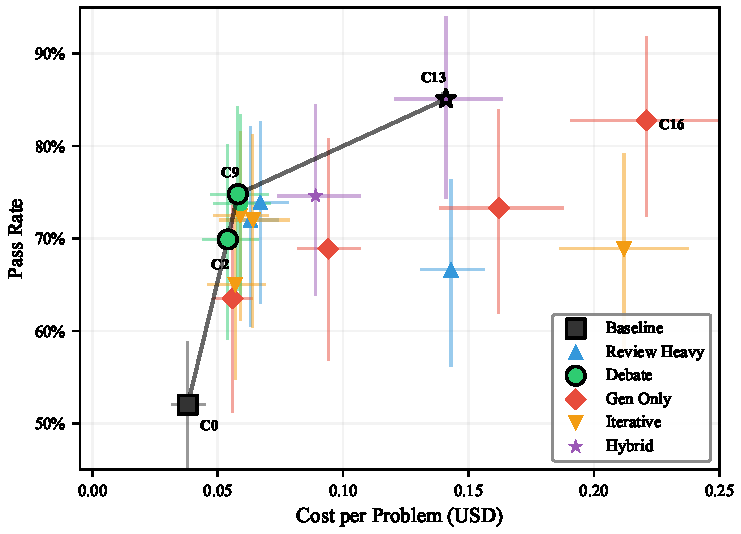
\includegraphics[width=\columnwidth]{figures/pareto_frontier.pdf}
\caption{Pareto frontier of pass rate versus cost per problem. Each point is a condition, colored by strategy family. The Pareto frontier (C0--C2--C9--C13) is connected by a solid line. C16 (best-of-7 generation) sits below and to the right of C13, worse on both dimensions. Error bars show 95\% bootstrap confidence intervals.}
\label{fig:pareto}
\end{figure}

The comparison between C13 and C16 on the calibration set is the cleanest test of the thesis. C13 runs 3 generations with 2 reviews each and a fix step per pipeline---3 generations, 6 reviews, 3 fixes. C16 runs 7 independent generations with no review. C13 achieves 85.1\% at \$0.141/problem. C16 achieves 82.8\% at \$0.221/problem. C13 is both cheaper and higher in point estimate. However, the 2.3pp pass rate gap is not statistically significant (Wilcoxon $p=0.53$, $n=30$ problems). The ``structure beats scale'' argument on the calibration set rests on Pareto dominance---C13 is cheaper \emph{and} has a higher point estimate---not on a statistically significant pass rate difference. The cross-domain result (Section~\ref{sec:crossdomain}) provides the statistically significant head-to-head: C13=93.0\% vs C16=64.7\% ($p=0.0002$ combined, driven primarily by MBPP where $p=0.002$).

The statistical comparison between baseline (C0) and the best hybrid (C13) is unambiguous: $p<0.0001$, effect size $r=0.85$. The baseline solves a problem 52.0\% of the time. The hybrid solves it 85.1\% of the time. For \$0.10 more per problem, you get 33 percentage points of pass rate.

Note on C16 pass@1: C16 achieves a pass@1 of 0.674---meaning each of its 7 individual pipelines passes at roughly the same rate as each of C13's 3 reviewed pipelines (0.689). C16 wins through volume (7 tickets at 67.4\% each versus 3 tickets at 68.9\% each), while C13 wins through quality. Both achieve high overall pass rates, but C13 does it at lower cost because it needs fewer pipelines to reach the same neighborhood.

\subsection{Where the Strategies Cluster}

The 17 conditions don't distribute uniformly across the pass rate--cost plane. They cluster by family in a revealing pattern. Generation-only conditions (C3, C6, C11, C16) form a line extending rightward---more generations buy more pass rate but at rapidly increasing cost, and the line sits below the Pareto frontier at every point. Review-heavy conditions (C1, C5, C8) cluster in the 66--74\% range regardless of how many reviews you add, suggesting diminishing returns from stacking reviews on a single generation. Iterative conditions (C4, C10, C12, C14) cluster similarly, with C14's aggressive fix strategy pushing cost up without proportional pass rate gain. Debate conditions (C2, C9, C15) show a tighter cost range (\$0.054--\$0.059) with meaningful pass rate variation (69.9--74.8\%), landing two of the four Pareto-optimal points.

The fact is, once you move beyond a single generation and a single review, the dominant strategy is always to add more \emph{pipelines} (generation + review), not more reviews per pipeline or more iterations within a pipeline. C13's architecture---three independent pipelines, each with its own review stage---captures this insight.

% ============================================================
\section{Replication and Generalization}
\label{sec:replication}

\subsection{Held-Out Replication}

I ran the Pareto-optimal conditions plus controls on 30 held-out competitive programming problems (2 replicas each) to test whether the calibration set findings generalize to unseen problems.

\begin{table}[t]
\centering
\caption{Held-out replication results (30 problems, 2 replicas per condition). All conditions show lower absolute pass rates than calibration (expected---the held-out set includes harder problems). The ordering C0 $<$ C9 $<$ C13 replicates.}
\label{tab:heldout}
\small
\begin{tabular}{lcccc}
\toprule
Condition & Calib. & Held-Out (SE) & $\Delta$ & $p$ (vs C0) \\
\midrule
C0  & 52.0\% & 38.7\% (8.8\%) & $-$13.3pp & -- \\
C2  & 69.9\% & 35.7\% (8.5\%) & $-$34.2pp & -- \\
C3  & 63.5\% & 40.1\% (8.7\%) & $-$23.4pp & -- \\
C9  & 74.8\% & 51.5\% (8.6\%) & $-$23.3pp & 0.028 \\
C10 & 72.5\% & 49.3\% (8.6\%) & $-$23.2pp & -- \\
C13 & 85.1\% & 55.6\% (8.7\%) & $-$29.5pp & 0.002 \\
C16 & 82.8\% & 48.9\% (8.7\%) & $-$33.9pp & -- \\
\bottomrule
\end{tabular}
\end{table}

C0 versus C13 on held-out problems: $p=0.002$, significant after Bonferroni correction. The core finding replicates---structured review beats baseline on unseen problems.

Two results deserve honest attention. First, C2 (debate with 2 reviewers) drops to 35.7\% on held-out---\emph{worse} than the 38.7\% baseline. The strategy that appeared Pareto-optimal on the calibration set actively hurts on harder problems. Its bootstrap Pareto inclusion was only 90.4\%, the lowest of the frontier conditions, and the held-out data confirms that instability. Second, C13's 6.7 percentage point advantage over C16 on held-out data (55.6\% vs 48.9\%) is directional but not statistically significant ($p=0.182$, Wilcoxon signed-rank). With 30 problems and 2 replicas, I do not have the statistical power to distinguish C13 from C16 on held-out competitive programming problems. The ``structure beats scale'' claim is strong on the calibration set and cross-domain benchmarks, and directional on held-out competitive programming.

The held-out Pareto frontier simplifies to C0 to C9 to C13. C2 drops off and C3 sits below the frontier---the strategies that were marginal on calibration data did not survive replication.

Rank correlation between the calibration and held-out orderings across the 7 tested conditions: Spearman $\rho=0.786$ ($p=0.036$), Kendall $\tau=0.714$ ($p=0.030$). The relative ordering of strategies is stable even when absolute pass rates shift.

\subsection{Cross-Model Validation}
\label{sec:crossmodel}

If the finding only holds for Claude Sonnet as generator, it is a finding about Sonnet, not about inference-time compute allocation. I tested two alternative generators---Qwen 2.5 Coder 32B and DeepSeek V3---on the 30 held-out problems with the same reviewer (Mercury-2) and fixer (Sonnet).

\begin{table}[t]
\centering
\caption{Cross-model results on held-out problems. All three columns show held-out rates for like-for-like comparison. The ordering C0 $<$ C9 $<$ C13 holds for all three generators. Reviewer and fixer are held constant; only the generator changes.}
\label{tab:crossmodel}
\small
\begin{tabular}{lccc}
\toprule
Cond. & Sonnet (SE) & Qwen (SE) & DeepSeek (SE) \\
\midrule
C0  & 38.7\% (8.8\%) & 0.0\% (0.0\%) & 25.6\% (7.1\%) \\
C9  & 51.5\% (8.6\%) & 40.5\% (8.4\%) & 40.3\% (8.2\%) \\
C13 & 55.6\% (8.7\%) & 53.2\% (8.5\%) & 57.3\% (8.2\%) \\
\bottomrule
\end{tabular}
\end{table}

\begin{figure}[t]
\centering
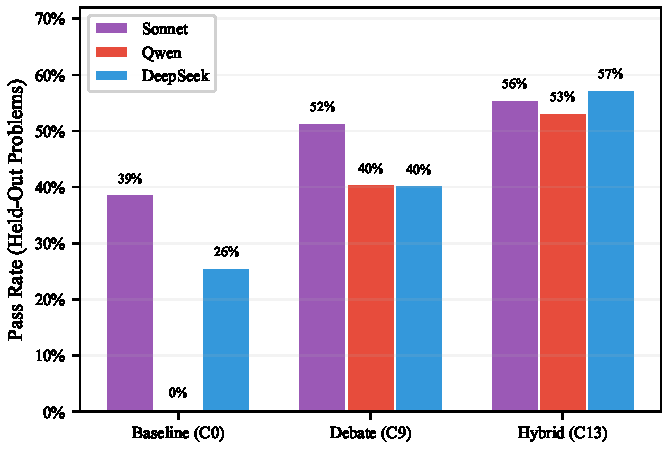
\includegraphics[width=\columnwidth]{figures/cross_model.pdf}
\caption{Cross-model validation on held-out problems. The ordering C0 $<$ C9 $<$ C13 holds for all three generators. Qwen 2.5 Coder 32B cannot solve a single problem alone (C0=0\%) but reaches 53.2\% through the review pipeline. Reviewer (Mercury-2) and fixer (Sonnet) are held constant. Error bars show $\pm$1 SE.}
\label{fig:crossmodel}
\end{figure}

\textbf{The confound I need to be upfront about.} In C9 and C13, the fixer is always Sonnet. So when Qwen generates code that fails and the review pipeline ``rescues'' it, what is actually happening is: Qwen provides a (bad) initial solution, Mercury reviews it, and Sonnet writes the fix. The review pipeline does not make Qwen a better generator. It routes Qwen's failed attempt through a strong reviewer and a strong fixer. The finding is that a weak-generator + strong-reviewer + strong-fixer pipeline works---the generator's role may be closer to ``providing a scaffold or failed attempt as context'' than ``generating a near-solution.'' This is still a meaningful result for inference-time compute allocation: it says that even a non-functional generator contributes value to a structured pipeline. The mechanism is unclear---it may be that the failed attempt provides useful context for the fixer, or it may be that Sonnet simply solves the problem independently when given the task description and review feedback as context. I ran a fixer ablation (Section~\ref{sec:ablations}) to test this: the fixer received the problem statement and reviewer bug list but not the generated code. On 30 held-out problems, the no-code condition achieved 48.6\% pass rate (SE=8.8\%) versus 55.6\% (SE=8.7\%) with code---a 7.0 percentage point drop---but a paired Wilcoxon signed-rank test yields $p=0.17$, failing to reach significance. The ablation is inconclusive: the data are consistent with the generator's code helping, but also consistent with no effect. The confound remains unresolved. But either way, this is not evidence that the review makes the original generator better.

The Qwen result is still striking on its own terms. Qwen 2.5 Coder 32B cannot solve a single competitive programming problem on its own---C0 = 0.0\%. Zero. But run that same model's output through a Mercury review and Sonnet fix pipeline, and it reaches 40.5\% (C9) or 53.2\% (C13). The only statistically tested pairwise comparison for Qwen is C0 vs C13 ($p<0.0001$). I do not have stored $p$-values for C0 vs C9 or C9 vs C13 on Qwen data, so I cannot claim all pairwise comparisons are significant.

DeepSeek V3 tells a different story with the same conclusion. DeepSeek solves problems independently (C0=25.6\%), so the review lift is genuine improvement, not rescue from total failure. All three pairwise comparisons are significant (paired Wilcoxon signed-rank tests on per-problem pass rates): C0 vs C9 ($p=0.0054$), C0 vs C13 ($p=0.0001$), C9 vs C13 ($p=0.0023$). The review pipeline adds value whether the generator is strong, weak, or non-functional---though in all cases, the fixer doing the actual repair work is Sonnet.

\subsection{Cross-Domain Validation}
\label{sec:crossdomain}

Competitive programming is a specific and demanding domain. Maybe structured review only helps because competitive programming problems have the kind of subtle edge cases that reviewers can catch. I tested on HumanEval and MBPP---standard benchmarks that are substantially easier---to check.

\begin{table}[t]
\centering
\caption{Cross-domain results (25 HumanEval + 25 MBPP problems, 2 replicas). SE computed on the combined 50-problem set. C16 included as the iso-cost control.}
\label{tab:crossdomain}
\small
\begin{tabular}{lcccc}
\toprule
Condition & HumanEval & MBPP & Combined (SE) \\
\midrule
C0  & 83.4\% & 40.0\% & 61.7\% (6.9\%) \\
C9  & 93.4\% & 82.0\% & 87.7\% (4.6\%) \\
C13 & 95.4\% & 90.7\% & 93.0\% (3.6\%) \\
C16 & 83.4\% & 46.0\% & 64.7\% (6.8\%) \\
\bottomrule
\end{tabular}
\end{table}

\begin{figure}[t]
\centering
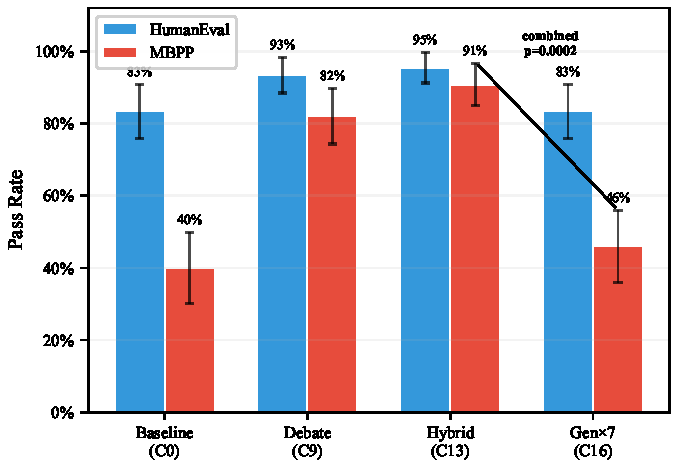
\includegraphics[width=\columnwidth]{figures/cross_domain.pdf}
\caption{Cross-domain validation on HumanEval (25 problems) and MBPP (25 problems). HumanEval shows a ceiling effect: C0 and C16 are tied at 83\%, and C16's 7 generations add nothing. The combined significance ($p=0.0002$) is driven primarily by MBPP, where C13 reaches 91\% vs.\ C16's 46\%. Error bars show $\pm$1 SE.}
\label{fig:crossdomain}
\end{figure}

The ordering holds on both benchmarks. C13 vs C16 combined: $p=0.0002$, significant after Bonferroni correction (4 comparisons, threshold $\alpha=0.0125$). Per-benchmark tests reveal where the signal comes from: on MBPP, C13 vs C16 is significant ($p=0.002$, 12 non-tied problems, C13 wins all 12). On HumanEval, C13 vs C16 is not significant ($p=0.109$, only 3 non-tied problems out of 25)---the ceiling effect leaves too few discriminating problems. The combined $p=0.0002$ is driven primarily by MBPP.

The MBPP result is the most dramatic: C0 at 40.0\% to C13 at 90.7\%---a 50.7 percentage point lift. HumanEval shows a ceiling effect: C0 is already at 83.4\%, and C16 (best-of-7) scores identically at 83.4\%. Seven attempts with no review beats one attempt with no review by exactly nothing on HumanEval. The problems Sonnet fails on HumanEval, it fails across all 7 attempts---suggesting the failures may reflect systematic rather than stochastic capability limitations, though I cannot distinguish this from correlated failures without per-attempt analysis. But review does---C13 pushes to 95.4\%. The ceiling effect on HumanEval means the benchmark cannot discriminate among strong strategies, which limits its diagnostic value, but it does show that generation scaling provides zero marginal value when the generator is already near ceiling.

\subsection{Matched-Fixer Experiment: Resolving the Fixer Confound}
\label{sec:matchedfixer}

The cross-model results in Section~\ref{sec:crossmodel} raise a question I flagged as open: when the fixer is always Sonnet, are the gains coming from the review structure or from Sonnet's superior fixing ability? To answer this, I ran a matched-fixer experiment where each generator model fixes its own code---Qwen fixes Qwen-generated code, DeepSeek fixes DeepSeek-generated code---with the same Mercury-2 reviewer.

\begin{table}[t]
\centering
\caption{Matched-fixer results on 30 held-out problems (2 replicas). ``Sonnet fixer'' columns reproduce Table~\ref{tab:crossmodel} data. ``Matched fixer'' columns show results where the generator's own model performs the fix.}
\label{tab:matchedfixer}
\small
\begin{tabular}{lcccc}
\toprule
Cond. & Qwen+Sonnet & Qwen+Qwen & DS+Sonnet & DS+DS \\
\midrule
C0  & 0.0\%  & 0.0\%  & 25.6\% & 25.6\% \\
C9  & 40.5\% & 0.0\%  & 40.3\% & 41.9\% \\
C13 & 53.2\% & 0.0\%  & 57.3\% & 51.8\% \\
\bottomrule
\end{tabular}
\end{table}

The results bifurcate sharply by generator capability.

\textbf{Qwen (weak generator): complete collapse.} When Qwen fixes its own code, the review pipeline produces nothing---C9=0.0\%, C13=0.0\%. Qwen cannot generate correct solutions, and it cannot fix its own incorrect solutions even with reviewer feedback. The entire 40.5--53.2 percentage point gain from the Sonnet-fixer pipeline was Sonnet solving the problems, not the review structure improving Qwen's code. An important caveat: this is a floor effect. Qwen scores 0\% at C0 on these problems. A model that cannot solve any problem cannot fix any problem, regardless of review quality.

\textbf{DeepSeek (capable generator): gains preserved.} When DeepSeek fixes its own code, the review pipeline retains its effectiveness. DeepSeek matched-fixer achieves C9=41.9\%, C13=51.8\%---compared to the Sonnet-fixer results of C9=40.3\%, C13=57.3\%. The C9 result is essentially unchanged, but C13 drops 5.5pp with matched fixer. The ordering C0 $<$ C9 $<$ C13 is preserved (25.6\% $<$ 41.9\% $<$ 51.8\%), indicating the review pipeline genuinely works for DeepSeek, but Sonnet-as-fixer provides an additional boost.

\textbf{Note on the primary pipeline.} The primary Sonnet pipeline (Sections~\ref{sec:results}--\ref{sec:crossdomain}) is itself a matched-fixer condition---Sonnet generates and Sonnet fixes. The matched-fixer experiment tests what happens when this property is extended to other generators.

\textbf{What this means for the thesis.} The ``structure beats scale'' finding has a prerequisite: the fixer must be capable enough to act on review feedback for the target task. The DeepSeek matched-fixer results suggest the review pipeline can genuinely amplify capable generators. The Qwen results are consistent with model substitution but cannot distinguish this from a floor effect, since Qwen has zero capability on these problems. The practical recommendation is unchanged: use structured pipelines, and ensure the fixer is at least as capable as the generator on the target task.

% ============================================================
\section{Why It Works: Reviews Improve Pipelines, Not Just Selection}
\label{sec:whyitworks}

There is a natural objection to the hybrid result: maybe C13 is just best-of-3 selection with extra steps. Three independent generations give you three shots at a correct answer. The reviews might be doing nothing---C13 might win because it generates three candidates, not because it reviews them.

The pass@1 data refutes this. Pass@1 measures whether an individual pipeline---a single generation plus its reviews and fix---produces a passing solution, before any cross-pipeline selection. If reviews were irrelevant, C13's pass@1 should match C6's pass@1, since both generate 3 independent solutions.

C13 pass@1: 0.689. C6 pass@1: 0.522. A 16.7 percentage point gap.

Both conditions generate three independent solutions. But C13 reviews each solution twice before fixing it. C6 does not. The review step makes each individual pipeline more likely to succeed, not just the overall ensemble. Reviews improve quality, not just selection odds.

\begin{figure}[t]
\centering
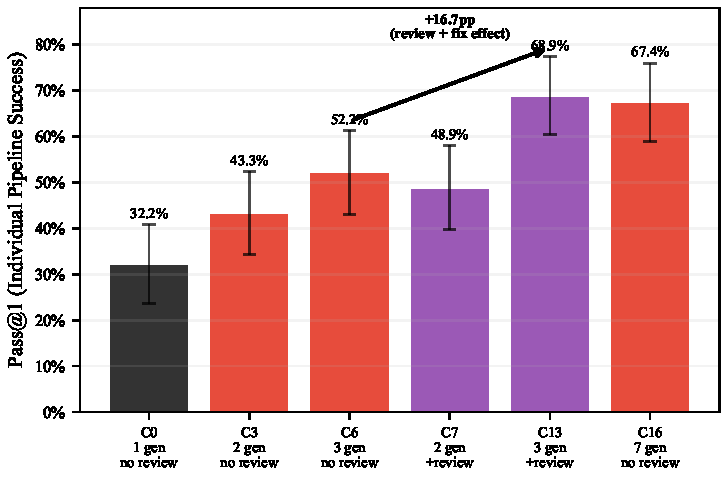
\includegraphics[width=\columnwidth]{figures/pass_at_1.pdf}
\caption{Pass@1 rates (individual pipeline success) for key conditions. C13 (3 gen + review + fix) and C6 (3 gen, no review) both generate 3 independent solutions, but C13's per-pipeline success rate is 16.7 percentage points higher, demonstrating that the review-and-fix step improves individual pipeline quality, not just ensemble selection. Note: for reviewed conditions, pass@1 reflects post-review-and-fix output; for gen-only conditions, it reflects raw generation quality. Error bars show $\pm$1 binomial SE ($n=30$ problems).}
\label{fig:passat1}
\end{figure}

For context, C16's pass@1 is 0.674---nearly matching C13's 0.689. This means each of C16's 7 unreviewed pipelines passes at almost the same rate as each of C13's 3 reviewed pipelines. The difference is that C13 achieves this per-pipeline quality through review rather than through having 7 independent chances, making it cheaper overall.

Generation-only scaling increases the number of independent attempts. Structured review increases the probability that each attempt succeeds.

% ============================================================
\section{Strategy Family Analysis and Ablations}
\label{sec:ablations}

\subsection{Difficulty Stratification}

I stratified the 30 calibration problems by C0 (baseline) pass rate into easy (C0 pass rate $>0.8$; 7 problems), medium (0.2--0.8; 17 problems), and hard ($<0.2$; 6 problems). Stratification uses only C0 performance to avoid circularity.

\begin{table}[t]
\centering
\caption{Pass rate by difficulty stratum on the calibration set, comparing selected conditions.}
\label{tab:difficulty}
\small
\begin{tabular}{lccccc}
\toprule
Difficulty & $N$ & C0 & C9 & C13 & C16 \\
\midrule
Easy   & 7  & 74.8\% & 83.5\% & 93.8\% & 98.2\% \\
Medium & 17 & 52.0\% & 79.8\% & 92.1\% & 85.9\% \\
Hard   & 6  & 25.3\% & 50.2\% & 55.0\% & 56.0\% \\
\bottomrule
\end{tabular}
\end{table}

\begin{figure}[t]
\centering
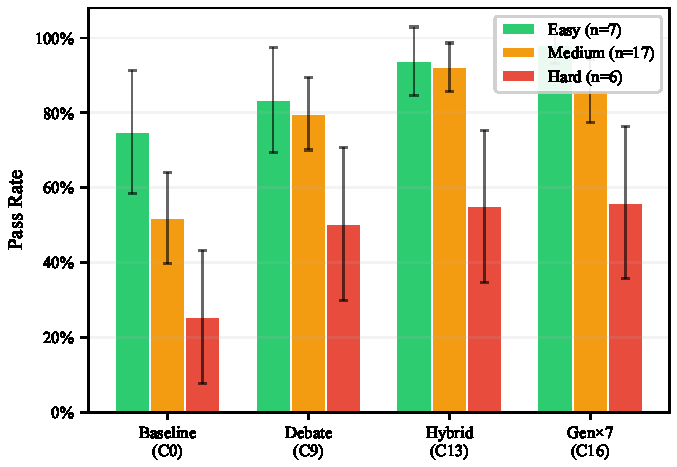
\includegraphics[width=\columnwidth]{figures/difficulty_stratification.pdf}
\caption{Pass rate by difficulty stratum for key conditions. C16 exceeds C13 on easy problems (98.2\% vs 93.8\%) and matches on hard problems (56.0\% vs 55.0\%). The medium stratum is where structured review provides its clearest advantage: C13 reaches 92.1\% vs C16's 85.9\%. Error bars show $\pm$1 binomial SE; note the small per-stratum sample sizes (easy $n=7$, medium $n=17$, hard $n=6$).}
\label{fig:difficulty}
\end{figure}

The gap between conditions narrows on easy problems---the generator is already good enough that review adds little---and on hard problems, where C13 and C16 converge near 55--56\%. The medium-difficulty stratum is where structured review provides its clearest advantage: C13 reaches 92.1\% versus C16's 85.9\%, a gap that aligns with the overall finding. C13 still reaches only 55.0\% on hard problems, which means roughly half of the hardest problems resist the full review pipeline. This is where diminishing returns set in: some problems require algorithmic insights that neither the generator nor the reviewer can provide, regardless of how many times you iterate.

\subsection{Review-Heavy Diminishing Returns}

The review-heavy family (C1, C5, C8) tests adding more reviews to a single generation: 1, 5, and 10 reviews respectively. Pass rates: C1=72.0\%, C5=66.6\%, C8=73.9\%. Cost: C1=\$0.063, C5=\$0.143, C8=\$0.067. There is no meaningful relationship between number of reviews and pass rate within this family. Adding 10 reviews instead of 1 to the same code does not reliably find more bugs---it just generates more noise. The reviewer sees the same code every time, and its ability to identify problems does not improve with repetition.

\subsection{Iterative Diminishing Returns}

The iterative family (C4, C10, C12, C14) tests review-fix loops: 2, 4, 8, and 2 (aggressive) iterations. Pass rates: C4=65.0\%, C10=72.5\%, C12=72.0\%, C14=68.9\%. C10 (4 iterations) and C12 (8 iterations) are nearly identical ($p=0.808$, $r=0.044$), suggesting the fix loop converges within 4 iterations. C14's aggressive fix strategy produces worse results at higher cost (\$0.212), confirming that more forceful intervention does not compensate for diminishing returns in the review-fix cycle.

\subsection{Debate Scaling}

The debate family (C2, C9, C15) tests multi-reviewer deliberation with 2, 3, and 5 reviewers. Pass rates: C2=69.9\%, C9=74.8\%, C15=73.8\%. C9 outperforms C15, suggesting that 3 reviewers is a sweet spot---5 reviewers adds no value and may introduce noise. Cost is nearly flat across the family (\$0.054--\$0.059 per problem), making debate the most cost-efficient review strategy.

\subsection{The Generation-Only Ceiling}

Generation-only conditions (C3, C6, C11, C16) show the scaling pattern documented by \citet{brown2024monkeys}: 2 gens = 63.5\%, 3 gens = 68.9\%, 5 gens = 73.3\%, 7 gens = 82.8\%. But cost scales linearly: \$0.056, \$0.094, \$0.162, \$0.221. The marginal pass rate per dollar spent decreases with each additional generation. By the time you reach C16 (7 gens), you are paying \$0.221/problem for 82.8\%---while C13 (3 gens + review) achieves 85.1\% at \$0.141. Generation scaling hits a ceiling that review-augmented strategies bypass.

\begin{figure}[t]
\centering
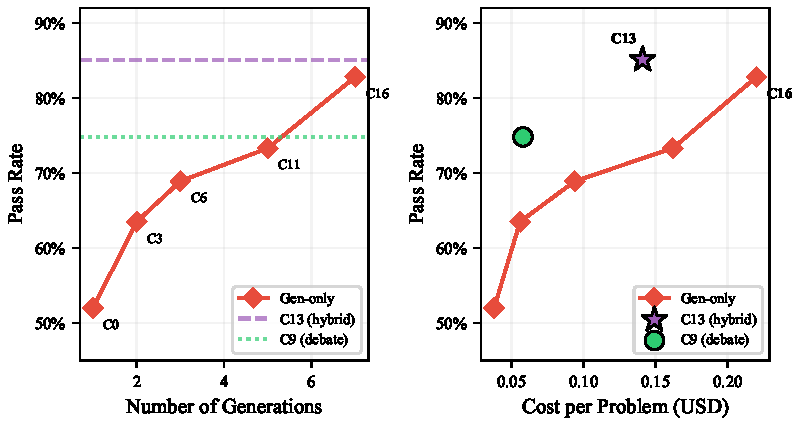
\includegraphics[width=\columnwidth]{figures/gen_only_scaling.pdf}
\caption{Generation-only scaling curve. \textbf{Left:} pass rate vs.\ number of generations. The curve flattens as $N$ increases. Dashed lines show C13 (hybrid) and C9 (debate) for reference. C0 (square marker) is the baseline---included as a natural anchor but plotted separately as it is not a gen-only condition. \textbf{Right:} pass rate vs.\ cost. C13 achieves higher pass rate than C16 at lower cost, though the difference is not statistically significant ($p=0.53$). Error bars show $\pm$1 SE.}
\label{fig:genscaling}
\end{figure}

\subsection{Temperature Sensitivity}

The generation-only conditions depend on temperature-driven diversity: higher temperature produces more diverse candidates, improving the odds that at least one is correct. If the default temperature (1.0) is suboptimal for generation-only scaling, the comparison against review strategies could be unfair.

I tested C16 at temperatures 0.4 and 0.8 on the 30 held-out problems (2 replicas each), compared against the existing C16 data at temperature 1.0.

\begin{table}[t]
\centering
\caption{Temperature sensitivity for C16 (best-of-7 generation) on held-out problems.}
\label{tab:temperature}
\small
\begin{tabular}{lcc}
\toprule
Temperature & Pass Rate (SE) & Runs \\
\midrule
0.4 & 46.4\% (8.9\%) & 59 \\
0.8 & 47.0\% (8.9\%) & 60 \\
1.0 (default) & 48.9\% (8.7\%) & 60 \\
\bottomrule
\end{tabular}
\end{table}

C16 pass rate is remarkably stable across temperatures: 46.4\% to 48.9\%, a 2.5pp range. The default temperature is not doing C16 any favors---lower temperatures produce nearly identical results. Temperature tuning cannot rescue generation-only scaling: even at the ``best'' temperature, C16 remains below C13 (55.6\%) on held-out data. The argument that ``C16 would win at a different temperature'' is empirically false.

\subsection{Cost Variance}

Most conditions exhibit high cost variance (coefficient of variation $>0.5$). C16 has the highest variance (CV=0.96, std=\$0.157), meaning its per-problem cost ranges from \$0.005 to \$0.707 depending on the problem. This matters for production deployment: a strategy with high cost variance is harder to budget for, even if its mean cost is acceptable. C13's cost variance is lower (CV=0.52, std=\$0.073), adding another practical advantage to the structured approach. Some of C13's cost variance comes from occasional runaway generations that hit the token limit (8,192 output tokens, costing ${\sim}$\$0.12 for a single generation versus ${\sim}$\$0.02 typical). These outliers inflate the per-problem cost but do not affect pass rates---the cost analysis uses actual measured costs, not trimmed means.

\subsection{Cost-Normalized Family Comparison}

At a fixed budget of \$0.06/problem, the family-level pass rates are: debate (0.738) $\approx$ hybrid (0.746) $>$ iterative (0.724) $\approx$ review-heavy (0.720) $\gg$ gen-only (0.641). Debate and hybrid tie at this budget level. Generation-only trails the field by 10 percentage points. The cheapest way to improve over baseline is debate; the most effective way regardless of cost is hybrid.

A note on the family taxonomy: the six strategy families (baseline, gen-only, review-heavy, debate, iterative, hybrid) are researcher-defined categories, not clusters discovered in the data. The labels are descriptive shorthand---``hybrid'' means ``multiple generations plus review,'' not a claim about a distinct mechanism. The cost-normalized comparison above and the iso-cost control (C16) are designed to test whether structure matters beyond total spend, but the family labels themselves carry no statistical weight.

\subsection{Fixer Ablation (Phase 6)}

A separate question from the matched-fixer experiment (Section~\ref{sec:matchedfixer}) concerns the generator's code itself: does it help the fixer, or does the fixer solve the problem from scratch given only the problem description and review feedback?

To test this, I ran C13\_nocode: the full C13 pipeline (3 generations, 2 reviews each), but the fixer receives only the problem statement and the reviewers' bug lists---not the generated code. Reviews still see the real code. The control is the existing C13 held-out data where the fixer sees everything, also with 2 replicas.

\begin{table}[t]
\centering
\caption{Fixer ablation results on 30 held-out problems (2 replicas each).}
\label{tab:fixer}
\small
\begin{tabular}{lccc}
\toprule
Condition & Pass Rate (SE) & Cost & Fix Rate \\
\midrule
C13 (with code) & 55.6\% (8.7\%) & \$0.141 & 23.2\% \\
C13\_nocode      & 48.6\% (8.8\%) & \$0.230 & 17.5\% \\
$\Delta$         & $-$7.0pp       & ---     & $-$5.7pp \\
\bottomrule
\end{tabular}
\end{table}

Paired Wilcoxon signed-rank test: $p=0.1716$. Not significant. Per-problem breakdown: the no-code condition performed worse on 7 problems, better on 2, and tied on 21. The large number of ties (21 of 30) reflects the bimodal nature of competitive programming---most problems are either solved by both conditions or neither---which limits the test's power to detect an effect of this magnitude.

The 7.0pp gap is directionally consistent with the generator's code helping the fixer. A paired Wilcoxon signed-rank test on per-problem pass rates (aggregating across replicas per problem) does not reach significance ($p=0.17$). The no-code condition still achieves 48.6\%---substantially above the C0 baseline of 38.7\%---meaning the fixer solves many problems from scratch given only the problem description and review context.

This result complements the matched-fixer finding (Section~\ref{sec:matchedfixer}): the fixer can often solve problems independently, which explains why the Sonnet-fixer pipeline works even with a non-functional generator like Qwen. The review serves as a structured problem description supplement, not necessarily as a fix guide for specific code.

% ============================================================
\section{What Doesn't Work, What I Don't Know, and What I Got Wrong}
\label{sec:limitations}

\subsection{Sample Size}

Thirty problems per benchmark. Three replicas per condition on the calibration set, two on held-out and validation sets. The effective sample size after accounting for the clustered design (ICC ranging from 0.14 to 0.74) is approximately 36--50. This produces wide confidence intervals---the standard errors in Tables~\ref{tab:calibration}--\ref{tab:crossdomain} range from 3.6\% to 8.8\%.

To make the uncertainty concrete: a 95\% CI for C13 on the calibration set is approximately 85.1\% $\pm$ 11.2pp (73.9\% to 96.3\%), and for C0 it is approximately 52.0\% $\pm$ 16.1pp (35.9\% to 68.1\%). These intervals do not overlap, consistent with the $p<0.0001$ result. But the C9 interval (74.8\% $\pm$ 13.9pp) overlaps heavily with C13, consistent with $p=0.014$ not surviving Bonferroni correction (12 comparisons, threshold $\alpha=0.0042$).

Here is what the statistics can and cannot distinguish. On the calibration set: C0 vs C13 ($p<0.0001$) and C0 vs C9 ($p=0.0002$) are solid. C9 vs C13 ($p=0.014$) does not survive correction---I cannot formally distinguish debate from hybrid on the calibration data. On held-out: C0 vs C13 ($p=0.002$) survives correction. C0 vs C9 ($p=0.028$) does not. C13 vs C16 is not significance-tested on held-out data---the 6.7pp gap could be noise. On cross-domain: C13 vs C16 ($p=0.0002$ combined, $p=0.002$ on MBPP alone, $p=0.109$ on HumanEval alone due to ceiling effect) is the cleanest separation in the entire study.

C13 has the highest ICC (0.74) and correspondingly the lowest effective $N$ (approximately 36), which means the condition I am most enthusiastic about is the one with the least statistical precision. I report this because it is true, not because I have a solution.

\subsection{Competitive Programming Bias}

The primary evaluation domain is competitive programming---algorithmic problems with comprehensive test suites, unambiguous specifications, and single-function solutions. Real-world software engineering involves ambiguous requirements, multi-file architectures, integration concerns, and test suites that the developer must write. I partially address this with HumanEval and MBPP, but those benchmarks share the same fundamental structure (function-level, fully specified, pre-written tests). Whether structured review helps with the kind of code that engineers actually write in production---multi-file changes, refactoring, API design---is an open question. SWE-bench \citep{jimenez2024swebench} would be a more appropriate evaluation surface for that question, and I have not tested on it.

All three benchmarks evaluate against pre-written test suites (typically 10--50 cases per problem). If generator models have encountered similar problems during training, they may produce solutions that pass the test suite while containing subtle errors that a larger or more adversarial test suite would catch. I have no way to measure this---the test suites are taken as given.

\subsection{Single-Turn Debate}

My ``debate'' conditions are not genuine debates. Multiple reviewers evaluate the code independently and sequentially; they do not respond to each other's arguments. A reviewer does not know what previous reviewers said. This means the debate conditions capture the value of reviewer diversity but not the value of adversarial argumentation. True multi-turn debate---where an attacker responds to a defender's rebuttals in real time---might produce meaningfully different results. I have not tested this.

\subsection{Reviewer Opacity}

Approximately 52.3\% of raw review responses from Mercury-2 were plain-text analysis rather than structured JSON. The verdict parsing system handles this gracefully (extracting pass/fail signals from unstructured text), but it means I cannot audit a majority of review decisions at the structured level. The verdict audit reports 0 mismatches among parseable responses, but this is a lower bound on review quality---I cannot verify what I cannot parse.

\subsection{Missing Fixer-Only Control}

The matched-fixer experiment (Section~\ref{sec:matchedfixer}) shows that the review pipeline works for capable generators, but does not fully decompose the fixer effect from the review effect. A clean decomposition would require a condition where the fixer receives the generated code but no review feedback---isolating whether the fixer improves code on its own, independent of review quality. Without this control, I cannot distinguish ``the review identifies real bugs that the fixer acts on'' from ``the fixer improves code regardless of review quality, and the review is an expensive no-op.'' The fixer ablation (Section~\ref{sec:ablations}) partially addresses this from the opposite direction---showing the fixer can solve problems without code---but the full decomposition remains open.

\subsection{Fixed Reviewer Model}

The reviewer (Mercury-2) is held constant across all experiments. I do not test alternative reviewer models---a limitation that leaves open the question of how reviewer capability affects pipeline performance. Mercury-2's specific strengths and weaknesses (e.g., its tendency to produce unstructured output) may not generalize to other review models.

\subsection{No Adaptive Selection}

In multi-generation conditions, candidate selection is based on test execution. In deployment, you might not have comprehensive test suites. A production version of this pipeline would need a selection mechanism that works without tests---learned verifiers \citep{cobbe2021training}, LLM-generated test filtering \citep{chen2023codet}, self-consistency voting, or confidence estimation. This study does not address selection without test suites because I wanted to isolate the effect of review structure from the confound of selection quality.

\subsection{Latency}

This paper reports dollar cost per problem but not wall-clock latency. The review pipeline adds sequential dependencies: a C9 run requires generation, then reviews, then a fix---steps that cannot be parallelized. C16's 7 independent generations can all run in parallel, reducing wall-clock time to roughly a single generation call. In serial execution, C9's total API latency (median 25.5s) is lower than C16's (median 136.2s), but this comparison is misleading: under realistic parallelization, C16 completes in roughly 22.6 seconds while C9 remains at 25.5 seconds. In latency-sensitive applications, the serialization cost of the review pipeline may outweigh its dollar cost advantage.

\begin{figure}[t]
\centering
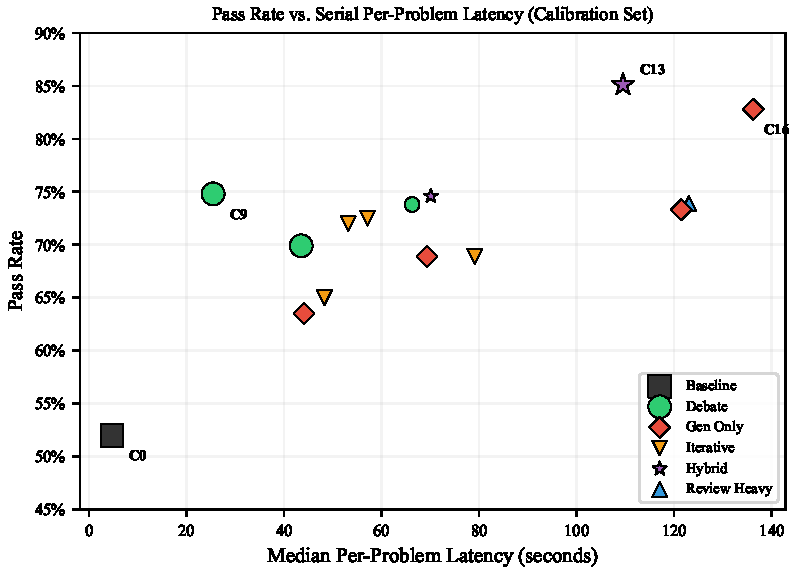
\includegraphics[width=\columnwidth]{figures/latency.pdf}
\caption{Pass rate versus serial (non-parallelized) per-problem latency on the calibration set. Under parallelization, C16's wall-clock time drops from $\sim$136s to $\sim$22.6s (a single generation call), while sequential pipelines like C9 (25.5s) cannot be similarly compressed. Serial latency favors review strategies; parallelized latency favors generation-only.}
\label{fig:latency}
\end{figure}

\subsection{Adaptive Design}

The calibration set design is adaptive: results from Studies A and B informed which conditions were included in Study C. This means the calibration results carry a multiple-testing burden beyond the Bonferroni correction applied to Study C's comparisons alone. The held-out, cross-model, and cross-domain experiments are the independent tests; the calibration results should be treated as hypothesis-generating for the conditions that were informed by earlier studies.

% ============================================================
\section{Conclusion}
\label{sec:conclusion}

At matched or lower cost, structured review achieves equal or higher pass rates than brute-force generation in every condition tested. C13 costs \$0.141/problem versus C16's \$0.221---36\% cheaper---while matching or exceeding C16's pass rate across calibration (85.1\% vs 82.8\%), held-out (55.6\% vs 48.9\%), and cross-domain data (93.0\% vs 64.7\%). Even where the pass rate differences are not statistically significant (held-out: $p=0.182$), the cost advantage alone justifies the structured approach. The ordering C0 $<$ C9 $<$ C13 holds across generators, across benchmarks, and across difficulty levels---strongly on calibration data and standard benchmarks ($p<0.001$), directionally on held-out competitive programming where statistical power limits what I can prove.

The matched-fixer experiment (Section~\ref{sec:matchedfixer}) adds an important nuance. DeepSeek's matched-fixer results---C0=25.6\%, C9=41.9\%, C13=51.8\%---demonstrate that the review structure genuinely works when the fixer is capable, independent of the fixer's superiority. Qwen's collapse to 0\% under matched fixing is consistent with model substitution, but the floor effect (Qwen=0\% at baseline) limits interpretation. The practical recommendation is unchanged---use structured pipelines with a capable fixer---but the mechanism depends on where the generator sits on the capability spectrum, and the boundary between ``capable enough to benefit'' and ``too weak'' is not characterized by this experiment.

Temperature sensitivity analysis confirms that generation-only scaling cannot be rescued by parameter tuning: C16 achieves 46.4\%--48.9\% across temperatures 0.4--1.0, never approaching the review-augmented conditions.

The interesting question is no longer whether to review, but how to optimize the pipeline further---alternative reviewers, the decomposition of fixer vs.\ review effects, multi-turn debate, and selection mechanisms that work without test suites. The 3,121-run dataset released with this paper provides the foundation for that work.

% ============================================================
\appendix

\section{Known Bugs and Corrections}
\label{app:bugs}

\textbf{Pipeline selection bug (fixed 2026-03-08).} Earlier versions of the analysis script read \texttt{pipelines[-1]} (the last pipeline's result) instead of \texttt{final\_test\_results} (the selected best result) for multi-generation conditions. This meant C3, C6, C7, C11, C13, and C16 were being evaluated on a single pipeline rather than the best-of-$N$ selection. All results in this paper reflect the corrected analysis.

\textbf{Difficulty stratification circularity (fixed 2026-03-09).} The original difficulty stratification used performance across all conditions to define easy/medium/hard categories, creating circular reasoning. The corrected stratification uses only C0 (baseline) performance: easy = C0 pass rate $>0.8$, medium = 0.2--0.8, hard $<0.2$. Result: 7 easy, 17 medium, 6 hard.

\textbf{Verdict parsing.} Approximately 52.3\% of Mercury-2 review responses (1,478 of 2,826) were plain-text analysis rather than structured JSON. The verdict parser extracts pass/fail signals from both formats. Among parseable structured responses, 0 mismatches were detected between the parser's interpretation and the structured verdict. Mismatches in plain-text responses cannot be systematically audited.

\section{Reproducibility}
\label{app:reproducibility}

All code, raw results (3,121 JSON files), and analysis scripts are available in the project repository. The experimental harness runs on a VPS with Docker sandboxing for test execution. The analysis script (\texttt{phase0\_analysis.py}) runs locally with standard Python dependencies (numpy, scipy, matplotlib, pandas).

\begin{figure}[t]
\centering
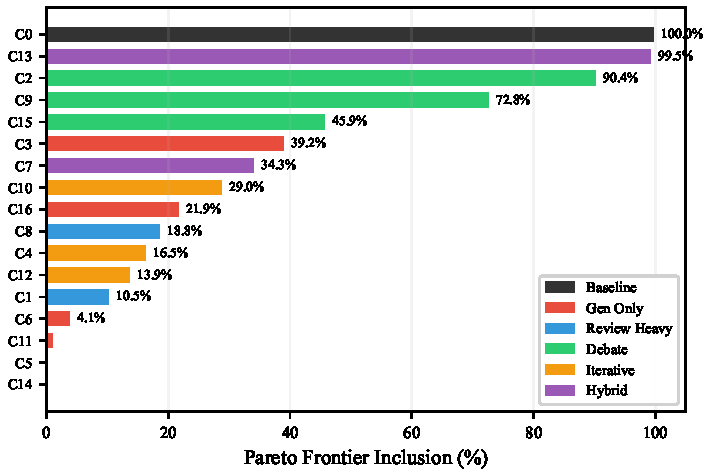
\includegraphics[width=\columnwidth]{figures/bootstrap_stability.pdf}
\caption{Bootstrap Pareto frontier inclusion rates (10,000 resamples). C0 and C13 appear on the frontier in $\geq$99.5\% of resamples. C9 appears 72.8\% of the time, reflecting instability in the mid-cost debate region. No generation-only condition exceeds 40\% inclusion.}
\label{fig:bootstrap}
\end{figure}

\bibliographystyle{plainnat}
\bibliography{references}

\end{document}
